\documentclass[journal, 10pt]{IEEEtran}
% *** CITATION PACKAGES ***
\usepackage{textcomp}
\usepackage{cite}

%\usepackage[numbers,sort&compress]{natbib}

\usepackage{filecontents}
\usepackage{amssymb}

% *** GRAPHICS RELATED PACKAGES ***
%
\ifCLASSINFOpdf
  \usepackage[pdftex]{graphicx}
\else
   \usepackage[dvips]{graphicx}
    % \DeclareGraphicsExtensions{.eps}
\fi
\usepackage{graphicx}

% *** MATH PACKAGES ***
\usepackage[cmex10]{amsmath}
% Also, note that the amsmath package sets \interdisplaylinepenalty to 10000
% thus preventing page breaks from occurring within multiline equations. Use:
%\interdisplaylinepenalty=2500 after loading amsmath to restore such page breaks as IEEEtran.cls normally

% *** ALIGNMENT PACKAGES ***
\usepackage{array}

% *** SUBFIGURE PACKAGES ***
\ifCLASSOPTIONcompsoc
  \usepackage[caption=false,font=normalsize,labelfont=sf,textfont=sf]{subfig}
\else
  \usepackage[caption=false,font=footnotesize]{subfig}
\fi
 %subfig.sty
% *** FLOAT PACKAGES ***
\usepackage{float}
\usepackage{stfloats}
\usepackage{hyperref}

\begin{document}
\title{Virtual Simulation for Testing a Vision-Based Autonomous Docking and Navigation Algorithm}

\author{John Karasinski, Christopher Lorenzen, and Melanie Stich\\Department of Mechanical \& Aerospace Engineering\\University of California, Davis\\Davis, CA, USA }

\maketitle

\begin{abstract}
With small failures leading to the loss of entire spacecraft, innovations in inspection methods are required.  Determining the viability of a proposed small satellite inspection free flyer with machine vision navigation is discussed and methods of testing the robustness of the system are developed.  Some past examples in the field are presented as well as their applicable contributions.  A baseline system using a traditional laser range finding position determination system is used as a comparison to rate the success of the proposed machine vision position determination system.  Two design aspects of the navigation control system are defined so that their alterations to the behavior of the craft can be identified.  A possible test environment and simulation methods are introduced to serve as a method of acquiring data to develop empirical cause and effect relationships between the different suggested control design parameters.
\end{abstract}

% Note that keywords are not normally used for peerreview papers.
\begin{IEEEkeywords}
robots, satellite
\end{IEEEkeywords}


\section{Introduction}

\subsection{Background}
In recent years the small satellite platform has increased in popularity. With the ability to launch multiple small satellites as a secondary payload and the relatively low development cost involved, they are one of the most viable testbeds for new technologies.  One great example of this is the class of satellites that adhere to the CubeSat standard~\cite{CubeSat}.  Although the small size limits their capabilities, CubeSat initiatives have made many projects possible due to the minimal costs required.  Higher fidelity projects usually require a larger volume to contain all desired systems.  There are several projects that use slightly larger free flyers that have produced unique navigation demonstrations such as AERCam Sprint~\cite{Aercam}, Mini-AERCam~\cite{MiniAercam}, and SPHERES (SPHERES was also used for many subsequent projects due to its modular nature)~\cite{SPHERES}.An obvious limitation to small satellites is the ability to fit all required architecture within the size restrictions set by the design.  One way to reduce the space required is to choose your subsystems such that some may fill multiple roles.  An example of this is to use a science instrument to also collect navigation data.  More specifically, to use an optical sensor that is needed to take stereoscopic visual recordings for inspection purposes to also determine position and attitude relative to a target.  To do this the image captured must be used in conjunction with a machine vision algorithm in order to estimate navigational parameters.

The decision to use stereoscopic visual sensors to inspect was largely in part to increase ease of inspection for a human operator.  Using stereo vision and full visual light spectrum, a more familiar virtual image is produced.  Technicians are able to view the subject as if it was in front of them allowing for quick and informed decision making.

Additionally if the inspector had the ability to dock to the target craft, this could greatly increase the effective mission operation time.  The inspector could refuel, recharge, and download data.  Instead of a small disposable craft that has a single use, it could become a long term asset and an integral part of the target crafts diagnostic routines.  Most current docking procedures utilize a laser range finder for determining distance.  Laser range finders have flight heritage and have moderate accuracy~\cite{Docking}.

\subsection{Motivation}
The advantages presented by the addition of an inspector satellite to a larger craft show the necessity for the development of this technology.  Whether the target craft is inhabited by astronauts or not it can still increase the probability of completing a mission successfully.

There are two main types of damage of concern.  The first cause of alarm is physical damage due to collision with orbital debris or micrometeorites.  The second thing to monitor is component failure.  Either of these events can be disastrous to a mission.  The best case scenario is that the craft is not inhabited and you only lose a multimillion dollar piece of equipment.  With inspection capabilities, damage and failures can be identified in a timely manner.  With more information about the problem area and additional time to deal with the issue, the possibility of salvaging the mission increases greatly.  There are even additional opportunities that arise if inspection capability was integrated with other projects like DARPA’s Phoenix Satellites~\cite{Phoenix}.  If damage can be known or if the specific component that failed can be identified then a satellite similar to the Phoenix system can dock with and repair or repurpose a damaged satellite.


Using the International Space Station as an example, NASA has showed concern for both damage types that could be seen with a visual inspector.  There have already been studies done trying to quantify the danger involved with debris collision~\cite{Risk}.  As seen in Figure~\ref{ISS_risk}, the impact risk for different parts of the station have already been determined and an inspection satellite could be made to center its efforts in patrolling high risk areas.  There have also been close calls due to component failures.  One such incident that required emergency extra-vehicular activity was when an ammonia pump developed a leak in may of 2013~\cite{Ammonia}.

\begin{figure}[tb]
\begin{center}
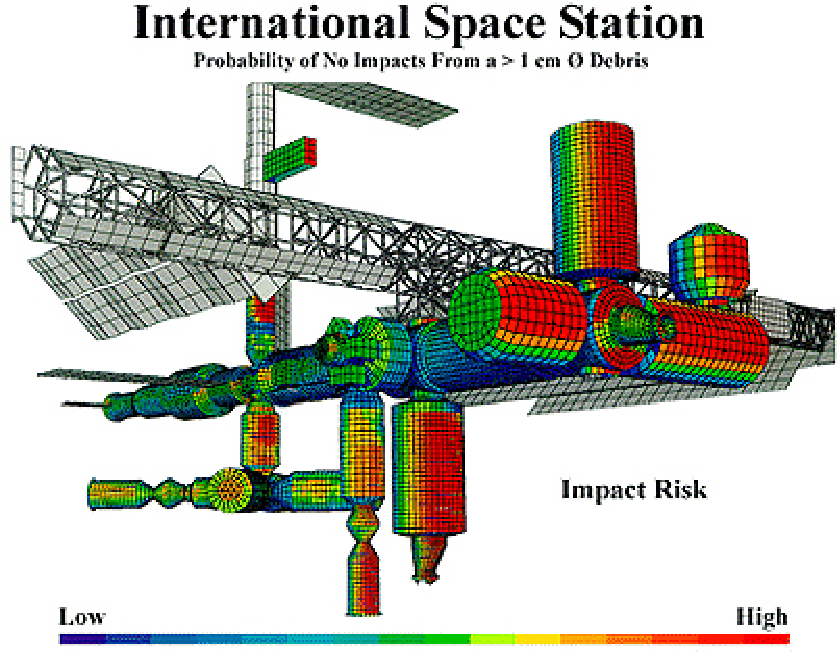
\includegraphics[width=0.4\textwidth]{figures/ISS_impact_risk}
\caption{Debris impact risk by region of the International Space Station}
\label{ISS_risk}
\end{center}
\end{figure}

Beyond the overall need for an inspection resource, there is also a driving factor to be as efficient as possible.  With increased navigational efficiency, it extends the life of the inspector as well as increases the data that is able to be gathered with each excursion.  As the inspection capability of the free flyer increases, the overall feasibility of the inspection mission increases.


\subsection{Objective}
% add that we will test using laser range finding
The purpose of this exercise is to create a simulation to test the viability and robustness of a machine vision based navigation system.  Several aspects will be modified to see if using stereoscopic cameras in conjunction with a machine vision algorithm is a viable option for a low cost inspection satellite.  To reduce costs, accuracy can be traded to reduce computational capabilities, battery power, and propellant needed.  When accuracy is reduced, chance of the inspector colliding with the subject increases, so a collision avoidance algorithm must also be tested.  With respect to the collision algorithm, the position error of the machine vision system must be analyzed to determine if a more accurate ranging device is required.

To test the viability of the machine vision system, a basic machine vision system will be compared to a more advanced laser range finding system.  Because of the limited processing power available, advanced machine vision systems are not possible.  The processing power required for a laser range finding system is minimal, so more advanced versions fit within the scope of the inspection craft.

When the study has been completed, we would like to answer:

\begin{quote}
``Given a small satellite with machine vision navigation, how does it perform versus a laser range finder based navigation and how does varying the path correction deadband width and position update frequency affect the fuel and time efficiency of traveling to a specific location near an object with a constant attitude and constant orbit?''
\end{quote}

The path correction deadband refers to the deviation that is allowed from the target trajectory before a correction burn is made while the position update frequency is how often the machine vision system determines, updates, and compares the inspection satellites position with the predicted position produced by the system dynamics and the inertial navigation system.  Under normal conditions, the only drift from the intended trajectory is from error or disturbances, but in this situation we also have drift due to the inspector and the target occupying different orbits.  This means that even with perfect planning and a perfect initial trajectory, corrections are required.  Since there is no way to circumvent course corrections, we must make our navigation scheme as efficient as possible.

With the concepts of deadband and update frequency explained, cause and effect relationships can be hypothesized but the weight of the interactions can only be seen from simulation.  There will be a lot of trade offs happening when the deadband width or update frequency are changed.  For example, a wider deadband will mean that the craft will make correction burns less often, but it will drift further off course than a slim deadband so that the corrections required will be larger.

% An example of a double column floating figure using two subfigures.
% (The subfig.sty package must be loaded for this to work.)
% The subfigure \label commands are set within each subfloat command,
% and the \label for the overall figure must come after \caption.
% \hfil is used as a separator to get equal spacing.
% Watch out that the combined width of all the subfigures on a
% line do not exceed the text width or a line break will occur.
%
%\begin{figure*}[!t]
%\centering
%\subfloat[Case I]{\includegraphics[width=2.5in]{Penguins}%
%\label{fig_first_case}}
%\hfil
%\subfloat[Case II]{\includegraphics[width=2.5in]{Penguins}%
%\label{fig_second_case}}
%\caption{Simulation results.}
%\label{fig_sim}
%\end{figure*}
%%

%\begin{table}[!t]
%% increase table row spacing, adjust to taste
%\renewcommand{\arraystretch}{1.3}
%% if using array.sty, it might be a good idea to tweak the value of
%% \extrarowheight as needed to properly center the text within the cells
%\caption{An Example of a Table}
%\label{table_example}
%\centering
%% Some packages, such as MDW tools, offer better commands for making tables
%% than the plain LaTeX2e tabular which is used here.
%\begin{tabular}{|c||c|}
%\hline
%One & Two\\
%\hline
%Three & Four\\
%\hline
%\end{tabular}
%\end{table}

\section{Literature Review}

\subsection{Overview of Small Inspection Satellites}
Over the past 20 years, there have been incredible advancements within the realm of semi-autonomous satellites. Beginning in 1997, the Autonomous Extravehicular Activity Robotic Camera Sprint (AERCam Sprint) was the first semi-autonomous satellite to demonstrate the use of a free-flying prototype camera aboard the International Space Station (ISS). While operating alongside STS-87 Mission Specialist Winston Scott, the AERCam Sprint flew under the remote-control guidance of Steve Lindsey for approximately 75 minutes, and relayed live television images to Columbia's Mission Control~\cite{Aercam, MiniAercam}. After successfully completing this experiment, researchers and analysts decided to incorporate a higher level of autonomy, and produced a second prototype known as the Mini AERCam in 2000. While this satellite never made it to space, the Mini AERCam underwent multiple tests on an air-bearing table and in an orbital test simulation facility at Johnson Space Center. This newly designed satellite was given automatic position hold, point-to-point maneuvering, and an additional camera to provide an orthogonal view, allowing astronauts to navigate the Mini AERCam with respect to the ISS. Through these multiple additions, researchers expanded the satellite's capability to encompass supervised autonomous and/or remotely piloted operations~\cite{MiniAercam, MiniAercam2}.

Later, in 2006 the first Synchronized Position Hold Engage Reorient Experiment Satellites (SPHERES), a self-contained nanosatellite made by MIT's Space Systems Laboratory, was launched to the ISS and taken to the US Laboratory. Since that time, this semi-autonomous satellite has been joined by two additional SPHERES, making this system the first consistent experimental nanosatellite testbed aboard the ISS. Unlike the AERCam Sprint and the Mini AERCam, SPHERES is a modular satellite where each system is self-contained in individual capsules. This configuration allows SPHERES to easily incorporate system expansions onto specific platforms, such as navigation, without needing to reconfigure the entire craft. Furthermore, its modularity helps researchers efficiently address system failures, making it easier for astronauts to perform on-site repairs. To navigate SPHERES within the ISS, the system utilizes wall-mounted ultrasonic beacons and corresponding ultrasonic receivers attached to the nanosatellite~\cite{SPHERES}. [When SPHERES looks to determine its location, it emits an infrared flash. Once emitted, the satellite waits for the wall-mounted beacons to emit corresponding ultrasonic pulses. After receiving these ultrasonic pulses, the satellite measures its range based on the pulse's time of flight, and can then calculate its relative position, attitude, and angular velocity~\cite{SPHERES, Vertigo1}.] This unique navigation system allows SPHERES to emulate a ``pseudo-GPS'' time-of-flight sensing system, and ultimately estimate its position, angular velocity, and attitude without the potential for signal interference and noise -- a challenge that has been previously encountered with GPS systems~\cite{Vertigo1}. Through this autonomous navigation and modular design, the SPHERES testbed has become a versatile platform for developing vision-based navigation algorithms, as well as anti-collision and formation flying algorithms. By allowing research teams to create algorithms that can then be uplinked to the SPHERES test system aboard the ISS, researchers can receive live feedback, and ultimately find the exact areas within their algorithms that need improvement.

\begin{figure}[tb]
\begin{center}
\includegraphics[width=0.4\textwidth]{figures/Spheres_Auto10.pdf}
\caption{SPHERES time-of-flight range measurements and wall-mounted ultrasound beacons.}
\label{spheres_plot}
\end{center}
\end{figure}

\subsection{SPHERES VERTIGO}
In 2008 the MIT Space Systems Laboratory began building an upgrade to the SPHERES system, known as the Low Impact Inspection Vehicle (LIIVe), as part of the Visual Estimation and Relative Tracking for Inspection of Generic Objects (VERTIGO) program. Once completed, this upgrade would later be attached to the existing SPHERES system and act as VERTIGO ``goggles,'' allowing SPHERES to perform vision-based navigation experiments in the microgravity environment aboard the ISS. After adjusting these VERTIGO Goggles to suit the ISS environment, the final system was upgraded to include two monochrome stereo cameras, two illuminating LEDs, a Via 1.2 GHz Via Nano processor, a 802.11n network card, and optics that included a larger aperture lens in a synchronized stereo configuration~\cite{SPHERES}-~\cite{Vertigo3}.

When the modified SPHERES VERTIGO was ready for experimentation, numerous flight algorithms were tested to demonstrate the spacecraft's complete autonomy. After ISS Expedition 34, it was confirmed that SPHERES VERTIGO was capable of autonomously conducting a circular orbit about an uncooperative object, while simultaneously maintaining a constant relative position between SPHERES VERTIGO and the target. This objective was achieved through the primary use of inertial sensors and cameras, and was considered an unprecedented success~\cite{Vertigo2, Vertigo3}.

While the SPHERES VERTIGO has already made considerable progress over the past few years, this advanced system continues to exhibit a perpetuating navigational limitation through the use of ultrasonic beacons and receptors.  As seen in Figure~\ref{spheres_plot}, the navigational hardware requires a total of five wall-mounted ultrasound beacons, confining the SPHERES VERTIGO system to one room. This ultimately  limits its overall use, and essentially forces SPHERES VERTIGO to remain as an experimental testbed~\cite{SPHERES, Vertigo 1, Vertigo2, Vertigo3}. Today, researchers are working to expand the system's navigational range by incorporating Google's Project Tango -- a mobile device that can track 3D motion allowing autonomous navigation within a building~\cite{Tango}. Researchers hope that once this hybrid Project Tango and SPHERES system, also known as ``Smart SPHERES,'' has been successfully implemented, the SPHERES nanosatellite will ultimately be able to traverse the entire ISS, performing interior maintenance and inspections.

\subsection{Collision Avoidance and Docking Algorithms}
Since the SPHERES nanosatellite's first microgravity guidance, navigation, and control experiment, there have been three classes of algorithms pertaining to collision avoidance and docking that have emerged: metrology, control, and autonomy~\cite{SPHERES_form}.

\subsubsection{Metrology Algorithms}
The metrology algorithms were implemented using a SPHERES-specific interface, and utilized a series of Extended Kalman Filters to obtain the system's state vector from the sensor outputs. While this approach has been typically utilized in position, attitude, and determination systems, recent literature has suggested that the second and third classes have demonstrated greater success and popularity in the areas pertaining to collision avoidance and docking algorithms~\cite{SPHERES_form}.

\subsubsection{Control Algorithms}
The control algorithm class involves both closed-loop controls and path-planning algorithms. One prominent control algorithm that has been frequently tested is the glideslope algorithm. This algorithm is a hybrid between a path-planning and a velocity-control algorithm, where the incoming spacecraft is given commands to slow its velocity as it approaches its target~\cite{SPHERES_form, SPHERES_micro, dist, virt_sim}. The glideslope algorithm was the first autonomous docking algorithm to successfully attach an incoming spacecraft to its tumbling target, and its simple, yet robust, controller makes this algorithm easy to store aboard SPHERES~\cite{SPHERES_micro}. Another algorithm that has also seen success is the ``safe'' trajectory algorithm. This innovative algorithm computes a pre-planned trajectory using the solution from a Mixed-Integer Linear Program, and, using this pre-computed trajectory, is able to optimize fuel and avoid incoming obstacles~\cite{SPHERES_micro}. However, while this algorithm is guaranteed to produce a safe trajectory, its overall complexity requires it to be computed on an external computer. Then once the computations have completed, the final trajectory is transferred to SPHERES. This entire computational process creates an approximate nine second delay, and can potentially create a catastrophic outcome if the spacecraft is tumbling towards an immediate collision. To remedy this solution, researchers have begun to trade trajectory and fuel optimality for computational time, and can reduce the total computation time to about $0.17$ seconds~\cite{SPHERES_micro}. Lastly, the close point of approach algorithm has been demonstrated to be both compact and computationally efficient, and has served as a background safety routine for the high school SPHERES Zero Robotics program~\cite{virt_sim}. While all three aforementioned algorithms have accurately performed numerous tests pertaining to collision avoidance and docking, each algorithm is associated with its own specific set of pros and cons. As it currently stands, researchers have yet to find a way to optimize fuel usage, pre-planned trajectories, and computational power, and thus must decide which factors are most important for any given mission~\cite{SPHERES_form, SPHERES_micro, dist, virt_sim}.

\subsubsection{Autonomous Algorithms}
Finally, the autonomous algorithm class is used to execute the control class algorithms and determine the current mode of operation~\cite{SPHERES_form}. As a result, the glideslope, ``safe'' trajectory, and close point of approach algorithms all utilize autonomy to properly perform their respective procedures. For this particular project, the authors recognize that autonomous collision avoidance and docking algorithms are an integral part in achieving a successful vision-based autonomous docking simulation. However, due to time limitations, the authors have chosen to simply focus on developing a virtual simulation for autonomous docking, and will readdress collision avoidance at a future date.

\subsection{Visual Simulations}

When testing a computer-vision based navigational algorithm, the first step is to simulate the algorithm in a comparable environment to test the system's design. For example, the research team at the West Virginia Robotic Technology Center (WVRTC) facility created a virtual environment to attempt to test their vision based pose estimation system, consisting of a monocular camera mounted to the tip of a robotic manipulator~\cite{virt_sim}. In doing so, the designers were able to exhibit how their system parameters effected their system's performance, and make dynamic modifications to their computer vision algorithms. Similarly, when the NASA JPL scientists simulated NASA's Mars Sample Return Mission, particularly the high-risk operation of capturing the Orbiting Sample, this research team performed numerous virtual simulations to test as many situations as possible, before implementing the final algorithm~\cite{mars}. As a result, advanced virtual simulations have become an integral procedure in emulating the system's environment, using tools such as EDGE and OpenCV, to aid in the detection of algorithmic deficiencies. The authors recognize that this is an optimal way for testing a vision-based autonomous navigation algorithm, and will thus utilize a virtual simulation to test and demonstrate the navigational and docking algorithm's capability.

\subsection{Literature Review Conclusions}
Since the AERCam Sprint, there have been numerous advancements pertaining to small semi-autonomous and autonomous satellites, particularly in the areas regarding guidance, navigation, and control. Through the glideslope, safe trajectory, and close point approach algorithms, researchers have attained many viable options for docking and collision avoidance, but there still remains room for improvement. With the need for both computational efficiency and vehicle safety, there remains a wide area of computer science that researchers are continuing to explore, to ultimately find a solution to this problem. However, the most intriguing aspect of these programs is the fact that all satellites, excluding the AERCam Sprint, have been solely implemented in interior environments, when the AERCam Sprint was originally designed to assist astronauts in Extra Vehicular Activities (EVA)~\cite{Aercam, MiniAercam}. While the MIT Space Systems Laboratory is the closest team to attaining a functioning exterior inspection satellite through their SPHERES-X proposal, there still remains a relatively open field that has yet to be explored~\cite{SPHERES}. In this paper, the authors hope to take preliminary steps towards creating an exterior inspection satellite by developing machine vision navigation algorithms that could later be applied to a completed satellite system.

\section{Design Specifications}
Assume that there is a preexisting small satellite with machine vision navigation capabilities, and the following features are attached to implement the autonomous machine vision algorithms:
\begin{itemize}
\item Two color stereo cameras attached to the side of the satellite.
\item A wide angle 2.8mm f/1.3 CCTV lens with manual iris and focus, capable of a 96$^{\circ}$ horizontal angle and a 71$^{\circ}$ vertical field of view.
\item Two illuminating light-emitting diodes.
\item A computer capable of 1.2 GHz x86 Via Nano Processor, 4GB RAM, 1 MB L2 Cache, SSE3.
\item A 802.11n network card.
\end{itemize}
\cite{Vertigo2, Vertigo3, virt_sim, lens}

For this simulation, assume that the physical dynamics of the satellite have been previously implemented in secondary algorithms, and thus have no impact on the machine vision based algorithm. Furthermore, assume that this small satellite has reaction control wheels for attitude control and a sufficient supply power to properly conduct all virtual test simulations.  Although the inspector will also have enough fuel, it will be considered finite to determine accuracy of the different control schemes.

*****ANYTHING ELSE YOU GUYS THINK WE SHOULD ADD???
%added and changed some words, hopefully that is alright -Chris

\section{The Environment}
\subsection{The Spacecraft Environment}
Space is an extremely dangerous environment with many challenges of different natures and magnitudes. Some effects on spacecraft can arise from radiation, space debris and meteoroid impact, upper atmospheric drag, spacecraft electrostatic charging, and many other factors. While the resulting dynamics of these phenomena have various degrees of effect on small spacecraft, these are outside the scope of this work. For the purposes of the study, all of these factors are ignored. It is assumed here that the spacecraft is operating under nominal conditions in an otherwise empty environment.

\subsection{Dynamical Equations of Motion} \label{cweqs}
The Clohessy-Wiltshire equations were used to model the dynamics of the spacecraft while it was in close proximity to the target vehicle. The Clohessy-Wiltshire equations describe a simplified model of orbital relative motion, in which the target is in a circular orbit, and the chaser spacecraft is in an elliptical or circular orbit. This model gives a first-order approximation of the chaser's motion in a target-centered coordinate system. It is used here in planning rendezvous of the chaser with the target~\cite{cw_eqs}.

These equations of motion can be expressed as
\begin{equation}
\begin{split}
\ddot{x} &= 3n^2 + 2n\dot y \\
\ddot{y} &= -2n\dot x \\
\ddot{z} &= -n^2z
\end{split}
\end{equation}
and have the closed form solution given by
\begin{equation}
\begin{split}
x(t) = (4-3 \cos{(nt)})x_0 &+ \frac{sin{(nt)}}{n}\dot x_0 + \frac{2}{n} (1 - \cos(nt))\dot y_0\\
y(t) = 6(\sin{(nt)}-nt)x_0 &+ y_0 \frac{-2}{n}(1 - \cos{(nt)})\dot x_0 \\
                         &+ \frac{4 \sin{nt} - 3nt}{n}\dot y_0 \\
z(t) = z_0 \cos{(nt)} &+ \frac{\dot z_0}{n} \sin{(nt)}
\end{split}
\end{equation}
where
\begin{equation}
n = \sqrt{\frac{\mu}{a^3_t}}
\end{equation}
and $a_t$ is the semi-major axis of the target vehicle's orbit and $\mu$ is the standard gravitational parameter.

\section{Simulation}

\begin{figure}[tb]
\begin{center}
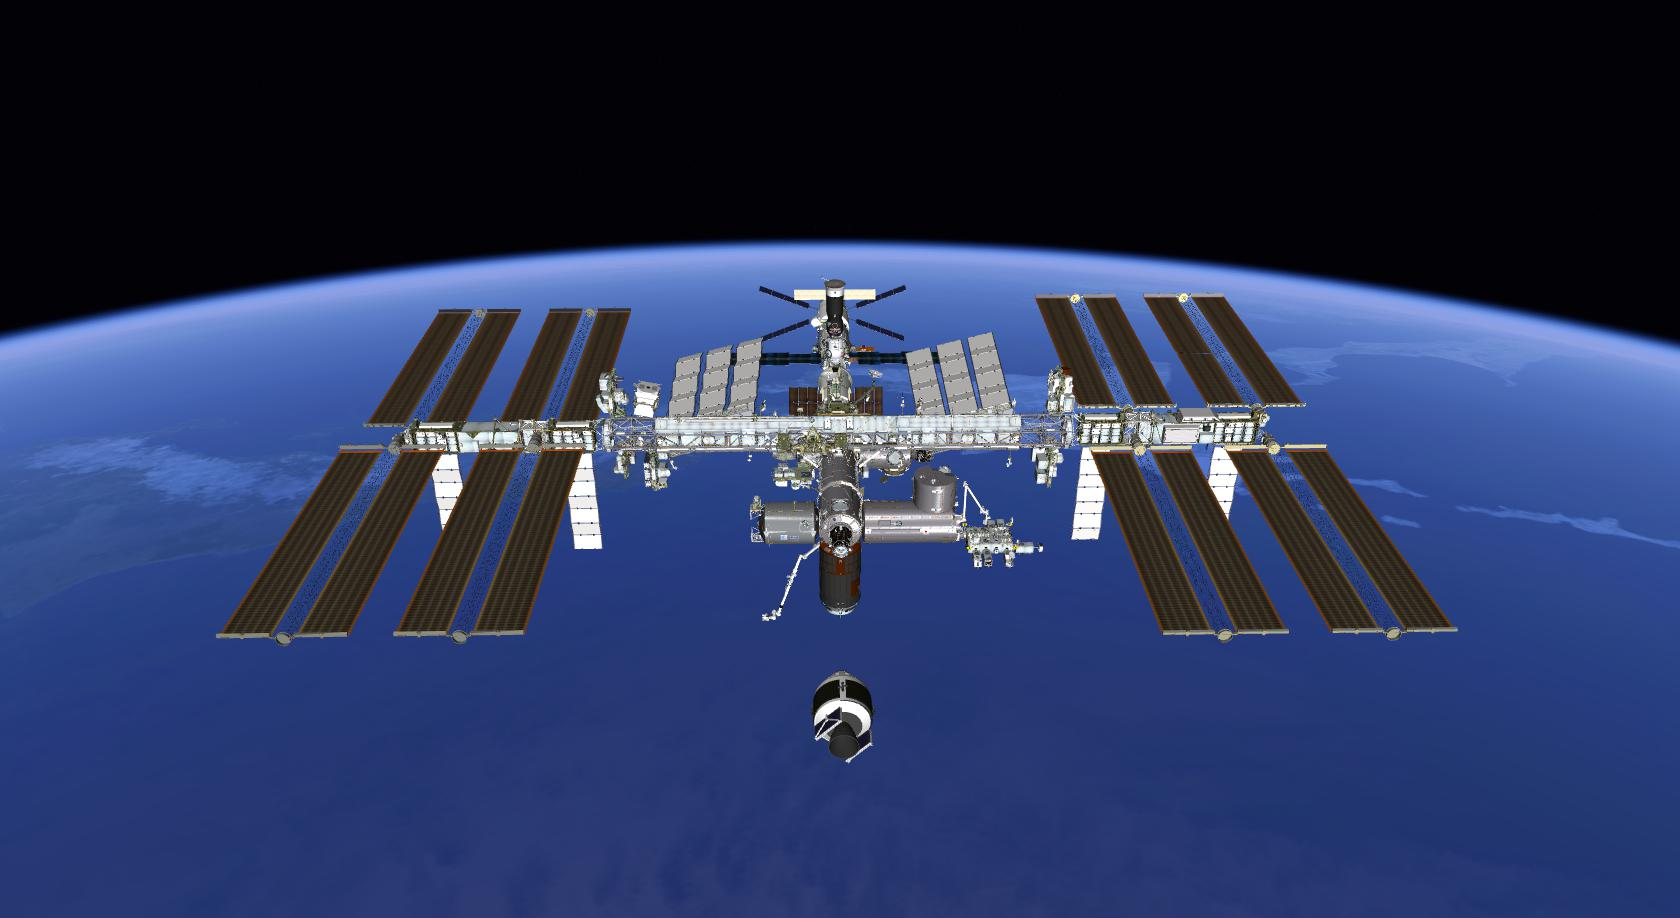
\includegraphics[width=0.5\textwidth]{figures/EDGE_ISS.jpeg}
\caption{Example EDGE visualization}
\label{edge_iss}
\end{center}
\end{figure}

The virtual simulation will be driven with a variety of software packages. The dynamics and control systems will be driven by several Python modules, while the visualization will be rendered in EDGE. EDGE is a graphics display tool developed at NASA's Johnson Space Center that combines key elements from graphics software developed for the space shuttle and the International Space Station programs and adapts them for integration with other engineering simulations and facilities~\cite{EDGE}.

EDGE makes use of a node tree to structure data, objects, and models. Each node has many properties, the most notable of which are position, orientation, and the node's parent. Each node's position and orientation are defined relative to it's parent's position and attitude. A node's parent can be changed to a different node, at which time the node's position and attitude are automatically updated to the correct values.

Three Python Python 2.7.9 scripts will be developed for use in the virtual simulation:
\begin{description}
    \item[\textbf{\textit{cv}}] \hfill \\
    A computer vision image processing module which takes advantage of OpenCV-Python version 2.4.9.
    \item[\textbf{\textit{dynamics}}] \hfill \\
    A dynamics and controls module.
    \item[\textbf{\textit{dcomm}}] \hfill \\
    A wrapper library developed to interface with EDGE's C++ DCOMM library.
\end{description}

\subsection{Python Modules}
\begin{figure}[b]
\begin{center}
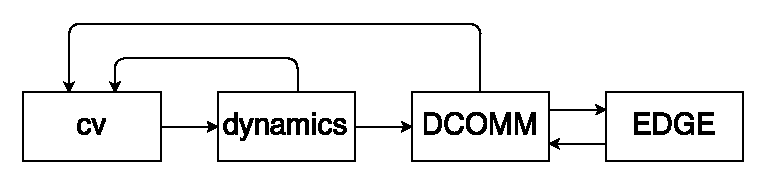
\includegraphics[width=0.5\textwidth]{figures/block.pdf}
\caption{Block diagram of software package interactions}
\label{block_diagram}
\end{center}
\end{figure}

\subsubsection{cv}
The \textit{cv} module takes advantage of Python bindings for OpenCV. OpenCV (Open Source Computer Vision) is a library of programming functions mainly aimed at real-time computer vision~\cite{opencv}. This module takes the live video feed from EDGE and attempts to identify features visible on the target spacecraft. The features of the target are supplied to the module a priori, and these descriptions were used to estimate the 3D pose of the target vehicle relative to the spacecraft's camera. This pose information is passed on to the \textit{dynamics} module

\subsubsection{dynamics}
The \textit{dynamics} module drives the dynamics and control of the simulation. The movement of the spacecraft around the target craft is modeled by the Clohessy-Wiltshire equations, see section~\ref{cweqs}. This module controls how the spacecraft operated in its different modes. Depending on pilot input, the spacecraft can navigate purely on line of sight, laser guided sensors to approach and hold a distance from a target, make use of the optical camera and machine vision to identify and dock with docking ports, or display guidance for a human pilot.

\subsubsection{DCOMM}
The \textit{DCOMM} module was previously developed to network between Python scripts and EDGE. The Python DCOMM interface allows a user to call various C++ functions from EDGE's DCOMM module and communicate with an EDGE server. Users can move and rotate nodes, and can also change a node's parents, units, and principal axis definitions. Commands to set the spacecraft's attitude and position were sent from the \textit{dynamics} module through DCOMM and passed on to EDGE. This module was also responsible for requesting and handing off the video feed from the EDGE server.

\subsection{Development Timeline}
Due to the short term nature of the project, an accelerated timeline has been planned. Weeks 1-3 were used for an initial literature and technology review. Key software technologies were chosen based on availability and ease of integration.

Weeks 4 and 5 will be used to develop core dynamics and control functions for the spacecraft. Development during this time will assume perfect knowledge of the relative distance and orientation of the target to test the core approach and hold algorithms. Data collected during this time will be used as a basis for comparison for the final trials where approach is made with noisy sensors.

Weeks 6 and 7 will be used to develop the algorithms necessary for the machine vision based 3D pose estimation. Once basic machine vision algorithms have been completed, integration between the two Python modules will begin. The primary task during this time will be to estimate the relative pitch of the target spacecraft (i.e., is the target above or below?). Once the relative attitude is estimated, functions developed in the control module will suggest appropriate rendezvous maneuvers. Yaw estimation will be investigated as a secondary priority, while roll estimation will be ignored due to the symmetry of the docking port.

Weeks 8 and 9 will be used for final integration of the submodules. At this time several trials will be ran to determine the effectiveness of each operational mode, and to determine which mode is the most effective. The effects of varying the deadband in each operational mode will be investigated to determine how frequently sensors must be activated. The effects of various levels of noise in the sensors will also be investigated.

%\section{Architectures}
%Use this section to describe which Joshi-defined architecture was implemented for our simulation (ie. Reactive, Deliberative Architecture, or both)
%**** DOES THIS SECTION WAIT TILL THE FINAL PAPER??
%
%\section{Techniques and Algorithms}
%not sure if this section should only be used for the final paper

%final paper only
%\section{Simulation Results and Discussion}

\section{Summary}
The conclusion goes here.


%final paper only
%\section{Future Work}

\nocite{*}
\bibliographystyle{IEEETran}
\bibliography{MAE252_MT_Paper}{}

\end{document}
